{\color{gray}\hrule}
\begin{center}
\section{System Design}
\bigskip
\end{center}
{\color{gray}\hrule}
\begin{multicols}{2}

\subsection{Architecture Overview}

The system architecture is designed around RESTful principles and leverages multiple Google Cloud Platform (GCP) services to achieve scalability, reliability, and high availability. The main components and their roles are outlined below:

\begin{itemize}
    \item \textbf{Google App Engine (GAE):} Hosts the REST API, implemented in Python 3 using the Flask web framework. It provides CRUD endpoints for managing patients, admissions, progress notes, media, and questions. GAE’s auto-scaling capability ensures the system adapts to varying loads efficiently.
    
    \item \textbf{Cloud SQL (MySQL):} A fully managed relational database used for storing structured data, including patients, admissions, progress, and questions. The schema is a simplified adaptation of MIMIC-III, consisting of tables such as \texttt{PATIENTS}, \texttt{ADMISSIONS}, \texttt{PROGRESS}, and \texttt{QUESTIONS}. Secure internal communication between GAE and Cloud SQL is achieved via Private IP configuration and the VPC Serverless Access Connector.
    
    \item \textbf{Cloud Storage Buckets:} Used for storing unstructured data such as images, videos, and documents associated with patients. The REST API provides endpoints for uploading and retrieving files, interfacing with Cloud Storage using GCP APIs.
    
    \item \textbf{Google Cloud Functions (FaaS):} Intended for periodic or compute-intensive tasks, such as updating a list of patients with the longest waiting times, which is derived from admission data. These functions are triggered via HTTP requests and interact with Cloud SQL in a serverless manner.
    
    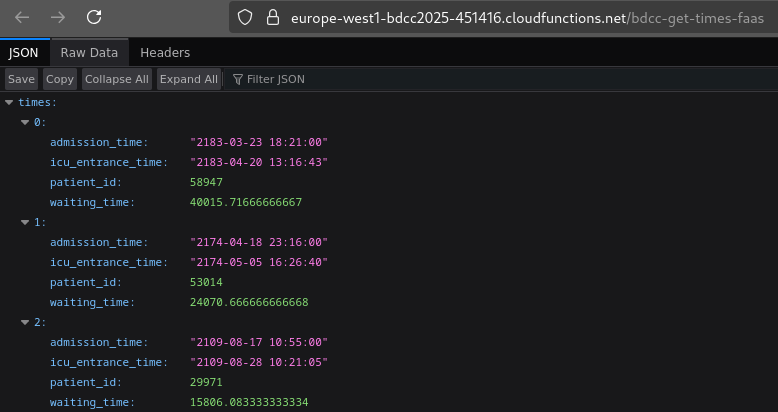
\includegraphics[width=\linewidth]{img/faas.png}
    
    
\end{itemize}

\subsection{Component Interactions}

To ensure seamless data flow and scalability, the system components are tightly integrated through a modular architecture. At the core, the REST API hosted on Google App Engine (GAE) is structured into route-specific Blueprints—\texttt{patient}, \texttt{admission}, \texttt{progress}, \texttt{media}, \texttt{question}, and \texttt{waiting time}. Each Blueprint encapsulates logic for handling specific entities, promoting modularity, maintainability, and clarity in code organization.

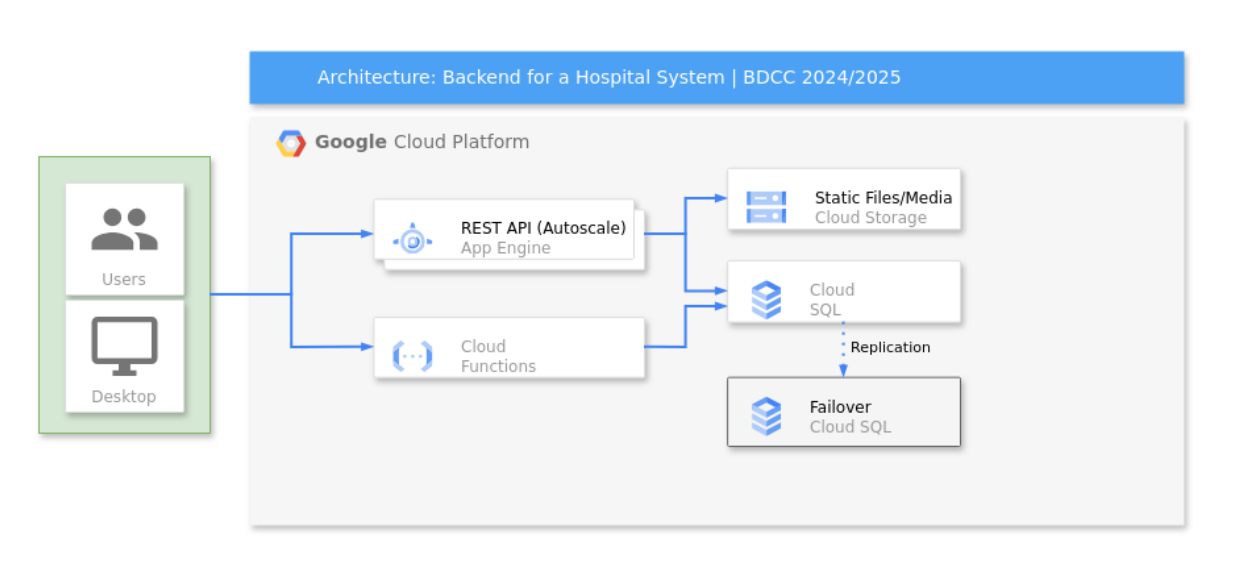
\includegraphics[width=\linewidth]{img/design.png}

A key feature of the system is its dynamic database connectivity, determined by the execution environment. In production, the system securely connects to Cloud SQL using the Cloud SQL Python Connector over a Private IP via the VPC Serverless Access Connector, with \texttt{pymysql} as the database driver. This connection logic is encapsulated in a reusable function that retrieves configuration from environment variables to initialize secure communication with the database.


\end{multicols}